%!TEX TS-program = luatex
%!TEX encoding = UTF-8 Unicode
%\documentclass[aspectratio=169,notes]{beamer}
\documentclass[aspectratio=169,handout]{beamer}
\usetheme[
outer/progressbar=foot,
outer/numbering=none
]{metropolis} 

\usepackage{pgfplots}
\usepackage{multimedia}
\usepackage[style=authortitle,backend=bibtex]{biblatex}
\addbibresource{references.bib}
\usepackage{tikz}
\usepackage{media9}
\usetikzlibrary{arrows,positioning}
\usetikzlibrary{calc} % for manimulation of coordinates
\usepgfplotslibrary{external} 
\tikzexternalize

\makeatletter
\def\@makefnmark{}
\makeatletter

\tikzset{
	%Define standard arrow tip
	>=stealth',
	%Define style for boxes
	mylabel/.style={text width=7em, text centered},
	mysmalllabel/.style={text width=7em, text centered},
	punkt/.style={
		rectangle,
		rounded corners,
		draw=black, very thick,
		text width=8em,
		minimum height=2.5em,
		text centered},
	punktt/.style={
		rectangle,
		draw=black, thick,
		text width=8em,
		minimum height=2.5em,
		text centered},
	% Define arrow style
	pil/.style={
		->,
		thick,
		shorten <=2pt,
		shorten >=2pt,}
}

\newcommand{\sectiondark}[1]{
	\metroset{background=dark} % change background theme according to manual
	\usebeamercolor[fg]{normal text}
	\section{#1}
	\metroset{background=light} % change background theme according to manual
	\usebeamercolor[fg]{normal text}
}

\makeatletter
%\setbeamertemplate{title}{
%	\raggedright%
%	\linespread{1.0}%
%	\inserttitle%
%	\par%
%	%\vspace*{0.5em}
%}
\setbeamertemplate{author}{
	\vspace*{2em}
	\begin{minipage}[t]{.2\textwidth}
		{\textbf{Candidate:}}
	\end{minipage}
	\begin{minipage}[t]{.8\textwidth}
	\insertauthor%
	\par%
	\end{minipage}
	\vspace*{0.25em}
}
\setbeamertemplate{date}{
	\hfill
	\insertdate%
	\par%
}
\setbeamertemplate{title page}{
	\begin{minipage}[b][\paperheight]{\textwidth}
		\vfill%
		\ifx\inserttitle\@empty\else\usebeamertemplate*{title}\fi
		\ifx\insertsubtitle\@empty\else\usebeamertemplate*{subtitle}\fi
		\usebeamertemplate*{title separator}
		\ifx\beamer@shortauthor\@empty\else\usebeamertemplate*{author}\fi
		\ifx\insertinstitute\@empty\else\usebeamertemplate*{institute}\fi
		
		\ifx\inserttitlegraphic\@empty\else\inserttitlegraphic\fi
		%\vspace*{1cm}
		\begin{minipage}[t]{.2\textwidth}
	    	{\small \textbf{Supervisors}:}%
	    	\par%
		\end{minipage}
		\begin{minipage}[t]{.8\textwidth}
			{\small Prof. Pietro Michiardi \hfill EURECOM, France}%
			\par%
			{\small Prof. Elena Baralis \hfill Politecnico di Torino, Italy}%
			\par%
		\end{minipage}
		
		\vfill
		\ifx\insertdate\@empty\else\usebeamertemplate*{date}\fi
		\vfill
		\vspace*{0mm}
	\end{minipage}
}
\makeatother

%\titlegraphic{%
%	\includegraphics[width=.2\textwidth]{example-image-a}\hfill\hfill
%	\includegraphics[width=.2\textwidth]{example-image-b}
%	
%}          % Use metropolis theme
\title{Model-Free Deep Reinforcement Learning algorithms applied to autonomous systems}
%\subtitle{Design and implementation of a control system for autonomous driving task of a small robot, exploiting state-of-the-art model-free deep reinforcement learning algorithms}
\date{\today}
\author{Piero Macaluso - s252894}
\setbeamercolor{background canvas in title}{parent=palette primary}
\setbeamercolor{progress bar}{use=palette primary}
% \titlegraphic{\hfill
\includegraphics[height=1.5cm]{logo.pdf}}
  
\begin{document}
\metroset{background=dark} % change background theme according to manual
\usebeamercolor[fg]{normal text}
\maketitle
\metroset{background=light} % change background theme according to manual
\usebeamercolor[fg]{normal text}
%\begin{frame}{Training Evolution}
%	\begin{figure}
%		\begin{tikzpicture}[scale=0.9]
%		\begin{axis}[mlineplot,legend pos=north west]
%		
%		\addplot table[x=Step,y=Value, col sep=comma] {plot/SAC/cozmodriver-v0/train/episode/mean.csv};
%		%\addlegendentry{Mean Reward of last 100 episode};
%		\addlegendentry{Mean $\mu$};
%		\addlegendentry{Area $[min, max]$};
%		\addlegendentry{Area $[\mu-\sigma, \mu+\sigma]$};
%		
%		\end{axis}
%		\end{tikzpicture}
%		\caption{Total reward for each episode. The maximum value of about 1200mm is at iteration 400.}
%		\label{fig:train_episode}
%		
%	\end{figure}
%\end{frame}
%\begin{frame}{Test Evolution}
%	\begin{figure}
%		\begin{tikzpicture}[scale=0.9]
%		\begin{axis}[mlineplot,legend pos=north west]
%		
%		\addplot table[x=Step,y=Value, col sep=comma] {plot/SAC/cozmodriver-v0/test/rewardMean/mean.csv};
%		%\addlegendentry{Mean Reward of last 100 episode};
%		\addlegendentry{Mean $\mu$};
%		\addlegendentry{Area $[min, max]$};
%		\addlegendentry{Area $[\mu-\sigma, \mu+\sigma]$};
%		
%		\end{axis}
%		\end{tikzpicture}
%		\caption{Mean Reward over 5 episode of test.}
%		\label{fig:test_episode}
%		
%	\end{figure}
%\end{frame}

%\begin{frame}{Mean 100 Episodes Evolution}
%	\begin{figure}
%		\begin{tikzpicture}[scale=0.9]
%		\begin{axis}[mlineplot,legend pos=north west]
%		
%		\addplot table[x=Step,y=Value, col sep=comma] {plot/SAC/cozmodriver-v0/train/meanLast100/mean.csv};
%		%\addlegendentry{Mean Reward of last 100 episode};
%		\addlegendentry{Mean $\mu$};
%		\addlegendentry{Area $[min, max]$};
%		\addlegendentry{Area $[\mu-\sigma, \mu+\sigma]$};
%		
%		\end{axis}
%		\end{tikzpicture}
%		\caption{Mean Reward over previous 100 episodes.}
%		\label{fig:train_mean100}
%		
%	\end{figure}
%\end{frame}
\begin{frame}
	\begin{center}
			\begin{minipage}{0.4\linewidth}
			\begin{center}
				\includegraphics[width=1\linewidth]{img/eurecom.png}
				\label{fig:eurecom}
			\end{center}
			\end{minipage}
			\begin{minipage}{0.4\linewidth}
							\begin{center}
				\includegraphics[width=1\linewidth]{img/polito.png}
				\label{fig:polito}
							\end{center}
			\end{minipage}
	
		This master thesis was developed at EURECOM (Sophia Antipolis, Biot, France)\\in collaboration with
		
		Prof. Pietro Michiardi (EURECOM)\\Prof. Elena Baralis (Politecnico di Torino)
	\end{center}
\end{frame}

\begin{frame}{Table of contents}
	\setbeamertemplate{section in toc}[sections numbered]
	\tableofcontents[hideallsubsections]
\end{frame}

\sectiondark{Reinforcement Learning Background}

\begin{frame}{Beyond supervised and unsupervised learning}
	\textbf{Supervised Learning}
		\begin{itemize}
			\item \textbf{Data}: $(x, y)$ where $x$ is data, $y$ is label
			\item \textbf{Goal}: Learn a function $f : x \rightarrow y$
			\item \textbf{Examples}: \textbf{Classification}, object detection, semantic segmentation, image captioning, ...
	\end{itemize}
	
		\begin{center}
			\begin{tikzpicture}
			\node[inner sep=3pt](imgcat) at (0,0) {\includegraphics[width=.25\textwidth]{img/cat.jpg}};
			\node[inner sep=3pt](label) at (5,0) {\textbf{CAT}};
				\draw[->, thick](imgcat.east) -- (label.west);
				\end{tikzpicture}
		\end{center}
		
	\end{frame}
	
	\begin{frame}{Beyond supervised and unsupervised learning}
		\textbf{Unsupervised Learning}
			
			\begin{itemize}
				\item \textbf{Data}: No more labels, just data.
				\item \textbf{Goal}: Learn some underlying hidden structure of the data. 
				\item \textbf{Examples}: Clustering, \textbf{dimensionality reduction}, feature learning, density estimation, ...
		\end{itemize}
		
		\begin{center}
				\includegraphics[width=0.6\linewidth,]{img/pca.png}
				\vspace{3mm}
				 \footcite{scholz2006approaches}
		\end{center}	
		
	\end{frame}

\begin{frame}{Reinforcement Learning}
	\onslide<1->{Problems involving an \alert<1-1>{\textbf{agent}}} \onslide<2->{interacting with an \alert<2-2>{\textbf{environment}}}\onslide<3->{, which provides numeric \alert<3-3>{\textbf{reward signals}}.}
	
	\onslide<4->{\textbf{Goal}: Learn how to take actions in order to maximize reward}
	\begin{center}
		\scalebox{0.9}{
		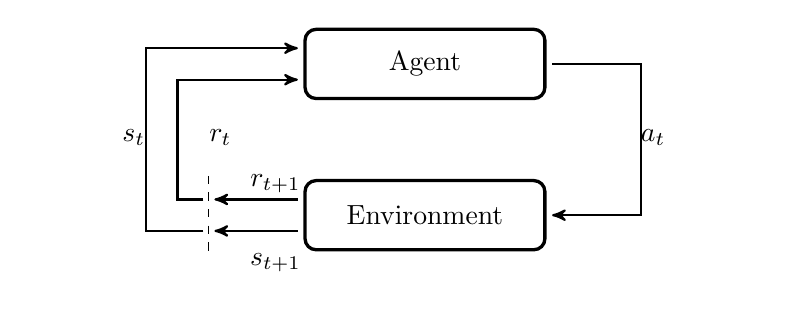
\begin{tikzpicture}
		% node Agent
		\node[punkt] (agent) {Agent};
			% node Environment
		\node[punkt, below=1cm of agent] (env) {Environment};
		% node a_t
		\node[mylabel, below right=0.25cm and 0cm of agent] (action) {$a_t$};
		% node s_t
		\node[mylabel, below left=0.25cm and 0.8cm of agent] (state) {$s_t$};
		% node r_t
		\node[mylabel, below left=0.25cm and -0.3cm of agent] (reward) {$r_t$};
		% node s_t+1
		\node[mylabel, above left=-1.3cm and -1cm of env] (state) {$s_{t+1}$};
		% node r_t+1
		\node[mylabel,above left=-.3cm and -1cm of env] (reward1) {$r_{t+1}$};
		\draw[pil]   (agent.east) -- ($(agent.east) + (1.2cm,0cm)$)  |-  (env.east);
		\onslide<3->{\draw[pil]   ($(env.west) + (0,-0.2cm)$) -- ($(env.west) + (-1.2cm,-0.2cm)$);
		\draw[pil]   ($(env.west) + (-1.2cm,-0.2cm)$) -- ($(env.west) + (-2cm,-0.2cm)$) |-($(agent.west) + (0,0.2cm)$);
		\draw[pil]   ($(env.west) + (0,+0.2cm)$) -- ($(env.west) + (-1.2cm,+0.2cm)$);
		\draw[pil]   ($(env.west) + (-1.2cm,+0.2cm)$) -- ($(env.west) + (-1.6cm,+0.2cm)$) |-($(agent.west) + (0,-0.2cm)$);
		\draw[dashed]  ($(env.west) - (1.2cm,-0.5cm)$) -- ($(env.west) - (1.2cm,0.5cm)$);}
		\end{tikzpicture}
		\footcite*{sutton2018reinforcement}
	}
	\end{center}

	
\end{frame}

%\begin{frame}{Reinforcement Learning Example}
%	
%	\onslide<1->{Problems involving a \alert{\textbf{Human}} interacting with \alert{\textbf{Earth}}, which provides \textbf{material reward}.}
%	\onslide<2->{}	\onslide<3->{}
%	
%\textbf{Goal}: Accumulate money for his/her future
%	\begin{center}
%		\scalebox{0.9}{
%			\begin{tikzpicture}
%			% node Agent
%			\node[punkt] (agent) {Human};
%			% node Environment
%			\node[punkt, below=1cm of agent] (env) {Earth};
%			% node a_t
%			\node<1-1>[mylabel, below right=0.25cm and 0.5cm of agent] (action) {Study};
%			\node<2-2>[mylabel, below right=0.25cm and 0.5cm of agent] (action) {Work};
%			\node<3-3>[mylabel, below right=0.25cm and 1.25cm of agent] (action) {Rob a Bank};
%			% node s_t
%			\node[mylabel, below left=-0.25cm and 1.75cm of agent] (state) {What the human sees and feels};
%			% node r_t
%			\node<1-1>[mylabel, below left=0.15cm and -1.1cm of agent] (reward) {$\{0,-10,10\}$€};			% node s_t+1
%			\node<2-2>[mylabel, below left=0.15cm and -1.1cm of agent] (reward) {$\{50,60\}$€};			% node s_t+1
%			\node<3-3>[mylabel, below left=0.15cm and -1.1cm of agent] (reward) {$100'000$€};			% node s_t+1
%			\node[mylabel, above left=-1.3cm and -1cm of env] (state) {};			% node r_t+1
%			\node[mylabel,above left=-.3cm and -1cm of env] (reward1) {};
%			\draw[pil]   (agent.east) -- ($(agent.east) + (1.2cm,0cm)$)  |-  (env.east);
%			\draw[pil]   ($(env.west) + (0,-0.2cm)$) -- ($(env.west) + (-1.2cm,-0.2cm)$);
%				\draw[pil]   ($(env.west) + (-1.2cm,-0.2cm)$) -- ($(env.west) + (-2cm,-0.2cm)$) |-($(agent.west) + (0,0.2cm)$);
%				\draw[pil]   ($(env.west) + (0,+0.2cm)$) -- ($(env.west) + (-1.2cm,+0.2cm)$);
%				\draw[pil]   ($(env.west) + (-1.2cm,+0.2cm)$) -- ($(env.west) + (-1.6cm,+0.2cm)$) |-($(agent.west) + (0,-0.2cm)$);
%				\draw[dashed]  ($(env.west) - (1.2cm,-0.5cm)$) -- ($(env.west) - (1.2cm,0.5cm)$);
%			\end{tikzpicture}
%		}
%	\end{center}
%	
%	
%\end{frame}

\begin{frame}{Reinforcement Learning involves}
\begin{itemize}
	\item {\textbf<2-2>{Optimization}}
	\item {\textbf<3-3>{Delayed Consequences}}
	\item {\textbf<4-4>{Exploration}}
	\item {\textbf<5-5>{Generalization}}
\end{itemize}
\end{frame}

\note[itemize]{
	\item Goal is to find an optimal way to make decisions or at least a very good strategy
	\item Decisions now can impact things much later... (Saving for retirement, robbing a bank)
	\item Agent as scientist, Learn to ride a bike by trying (and failing), Decisions impact what we learn about
	\item Images and possibilities are enormous
}

\begin{frame}{Components of the Agent}
	\begin{itemize}
		\item{\textbf{Policy}:  agent’s behaviour function}
		\begin{equation*}
			\begin{aligned}
			\text{\textbf{Deterministic}: }& \pi(s) = a \\
			\text{\textbf{Stochastic}: }& \pi(a|s) = \mathbb{P}[A_t = a | S_t = s]
			\end{aligned}
		\end{equation*}
		\item{\textbf{Value Function}:  agent’s behaviour function}
				\begin{equation*}
				\begin{aligned}
				\text{\textbf{State Value}: }& V^\pi(s) = \mathbb{E} \Bigg[\sum_{t \ge 0} \gamma^k r_t|s_0 = s, \pi\Bigg]\\
				\text{\textbf{Action Value}: }& Q^\pi(s,a) = \mathbb{E} \Bigg[\sum_{t \ge 0} \gamma^k r_t \big| s_0 = s, a_0 = a, \pi\Bigg]\\
				\end{aligned}
				\end{equation*}
		\item{\textbf{Model}:  agent’s representation of the environment}
	\end{itemize}
	
\end{frame}

\begin{frame}{Categorizing Reinforcement Learning agents}
	\begin{columns}
		\begin{column}{0.5\linewidth}
			\begin{itemize}
				\item \textbf{Value Based}
				\begin{itemize}
					\item{\textcolor{lightgray}{No Policy (implicit)}}
					\item{Value Function}
				\end{itemize}
				\item \textbf{Policy Based}
				\begin{itemize}
					\item{Policy}
					\item{\textcolor{lightgray}{No value function}}
				\end{itemize}
				\item  \alert<2->{\textbf{Actor Critic}}
				\begin{itemize}
					\item{Policy}
					\item{Value function}
				\end{itemize}
			\end{itemize}
		\end{column}
		\begin{column}{0.5\linewidth}
			\begin{itemize}
				\item \alert<2->{\textbf{Model Free}}
				\begin{itemize}
					\item{Policy and/or value function}
					\item{\textcolor{lightgray}{No Model}}
				\end{itemize}
				\item \textbf{Model Based}
				\begin{itemize}
					\item{Policy and/or value function}
					\item{Model}
				\end{itemize}
			\end{itemize}
		\end{column}
	\end{columns}
\end{frame}



\begin{frame}{Reinforcement Learning aim}
	\begin{center}
	\includegraphics[width=0.8\linewidth]{img/decision.png}
	
	\textbf{Learn} to make \textbf{good} \textbf{sequences of decisions}.
	
	\onslide<1->{Fundamental challenge in artificial intelligence and machine learning is learning to make good decisions under uncertainty.}
\end{center}
\end{frame}

\begin{frame}{Let's go Deep!}
	
	\alert{\textbf{Google DeepMind's Deep Q-learning playing Atari Breakout}}
	
	\url{https://www.youtube.com/watch?v=V1eYniJ0Rnk}
	
	\centering
%	\includemedia[
%	addresource=video/deepmindatari.mp4,
%	activate=pageopen,transparent,
%	passcontext,
%	flashvars={source=video/deepmindatari.mp4},
%	width=0.8\linewidth, height=0.45\linewidth
%	]{\includegraphics{video/deepmindatari.jpg}}{VPlayer.swf}%
	\footcite*{mnih2013playing}
\end{frame}

\sectiondark{Reinforcement Learning for Autonomous Systems}
\begin{frame}{State-of-the-art Autonomous Driving Systems}
	\begin{center}
		\includegraphics[width=0.9\linewidth]{img/sensors.png}
	\end{center}
\end{frame}
\begin{frame}{Deep Learning for autonomous vehicles}
	\begin{center}
		\includegraphics[width=0.9\linewidth]{img/detection.jpg}
	\end{center}
\end{frame}
\begin{frame}{State-of-the-art Autonomous Driving Systems}
	\onslide<1->{}
		\onslide<2->{}
	\begin{center}
	\scalebox{0.8}{
	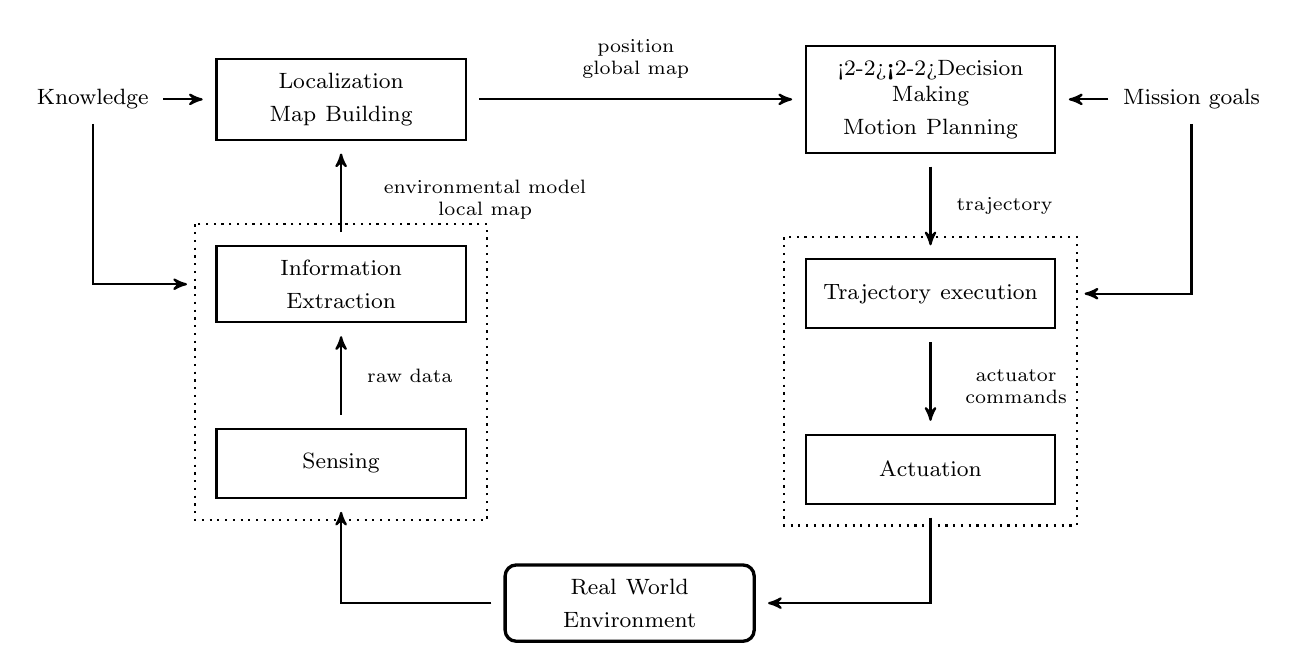
\begin{tikzpicture}
	\node[outer sep=2pt] (knowledge) {\footnotesize Knowledge};
	\node[punktt,inner sep=5pt,outer sep=5pt,right=0.5cm of knowledge] (localization) {\footnotesize Localization Map Building};
	\node[punktt,inner sep=5pt,outer sep=5pt,below=1cm of localization] (information) {\footnotesize Information Extraction};
	\node[punktt,inner sep=5pt,outer sep=5pt,below=1cm of information] (sensing) {\footnotesize Sensing};
	
	\draw[->, thick](knowledge.east) -- (localization.west);
	\draw[->, thick](sensing.north) -- (information.south) node [midway, right=0.2cm] {\scriptsize raw data};
	\draw[->, thick](information.north) -- (localization.south) node [midway, above right=-0.5cm and 0.2cm] {\scriptsize {\begin{tabular}{c}
			environmental model \\
			local map \\
			\end{tabular} }};
	\draw[->, thick](knowledge.south) |- ($(information.west) + (-0.2,0)$);
	\draw[black,thick,dotted] ($(information.north west)+(-0.1,0.1)$)  rectangle ($(sensing.south east)+(0.1,-0.1)$);
	
	\node[outer sep=2pt, right=12cm of knowledge] (mission) {\footnotesize Mission goals};
	\node[punktt,inner sep=5pt,outer sep=5pt,left=0.5cm of mission] (decision) {\footnotesize \alert<2-2>{\textbf<2-2>{Decision Making}} \\ Motion Planning};
	\node[punktt,inner sep=5pt,outer sep=5pt,below=1cm of decision] (trajectory) {\footnotesize Trajectory execution};
	\node[punktt,inner sep=5pt,outer sep=5pt,below=1cm of trajectory] (actuation) {\footnotesize Actuation};
	
	\node[punkt,inner sep=5pt,outer sep=5pt,below right=0.5cm and 0.15cm of sensing] (environment) {\footnotesize Real World Environment};
	
	\draw[->, thick](mission.west) -- (decision.east);
	\draw[->, thick](decision.south) -- (trajectory.north) node [midway, right=0.2cm] {\scriptsize trajectory};
	\draw[->, thick](trajectory.south) -- (actuation.north) node [midway, above right=-0.5cm and 0.1cm] {\scriptsize {\begin{tabular}{c}
			actuator \\
			commands \\
			\end{tabular} }};
	\draw[->, thick](mission.south) |- ($(trajectory.east) + (+0.2,0)$);
	\draw[black,thick,dotted] ($(trajectory.north west)+(-0.1,0.1)$)  rectangle ($(actuation.south east)+(0.1,-0.1)$);
	
	\draw[->, thick](localization.east) -- (decision.west) node [midway, above=0.1cm] {\scriptsize {\begin{tabular}{c}
			position \\
			global map \\
			\end{tabular} }};
		
	\draw[->, thick](actuation.south) |- (environment.east);
	\draw[->, thick](environment.west) -| (sensing.south);

	\end{tikzpicture}}
	\end{center}
\end{frame}

\begin{frame}{Learning to drive in a Day}
	
	\alert{\textbf{Learning to drive in a day}}
	
	\url{https://www.youtube.com/watch?v=eRwTbRtnT1I}
	
	\footcite*{kendall2018learning}
	
	\centering
%	\includemedia[
%	addresource=video/learningToDriveInOneDay.mp4,
%	activate=pageopen,transparent,
%	passcontext,
%	flashvars={source=video/learningToDriveInOneDay.mp4},
%	width=0.8\linewidth, height=0.45\linewidth
%	]{\includegraphics{video/learningToDriveInOneDay.jpg}}{VPlayer.swf}%

\end{frame}

\begin{frame}{Learning to Drive like a Human}
	
	\alert{\textbf{Urban Driving with End-to-End Deep Learning}}
	
	\url{https://www.youtube.com/watch?v=26Or4QbLbMM}
	
	\footcite*{wayve2019human}
	
	\centering
%	\includemedia[
%	addresource=video/drivingLikeHuman.mp4,
%	activate=pageopen,transparent,
%	passcontext,
%	flashvars={source=video/drivingLikeHuman.mp4},
%	width=0.8\linewidth, height=0.45\linewidth
%	]{\includegraphics{video/drivingLikeHuman.jpg}}{VPlayer.swf}%

\end{frame}

\begin{frame}{Model-Free Actor Critic methods}
	\begin{columns}
		\begin{column}{0.5\linewidth}
			\metroset{block=fill}
			\begin{exampleblock}{Critic Network}
				Estimates the value function. This could be the action value $Q$ or state value $V$.
			\end{exampleblock}
			\begin{exampleblock}{Actor Network}
				Updates the policy distribution in the direction suggested by the Critic (such as with policy gradients).
			\end{exampleblock}
		\end{column}
	\begin{column}{0.5\linewidth}
		\centering
		\includegraphics[width=0.8\linewidth]{img/actor_critic.png}
	\end{column}
	\end{columns}
		\footcite*{sutton2018reinforcement}

\end{frame}

\begin{frame}{Model-Free algorithms exploited}
	\centering
	\textbf{Deep Deterministic Policy Gradient (DDPG)}
	\begin{itemize}
		\item DDPG is an off-policy algorithm.
		\item Ornstein–Uhlenbeck process noise for exploration
		\item Countinuous action spaces
	\end{itemize}
	\textbf{Soft Actor-Critic (SAC)}
	\begin{itemize}
		\item SAC is an off-policy algorithm which exploits entropy-regularized reinforcement learning
		\item Auto-tune parameters: Less hyper-parameters, less tuning
		\item Suitable for Real-World Experiments
	\end{itemize}
	\footcite*{lillicrap2015continuous}
	\footcite*{haarnoja2018alg}
\end{frame}

\sectiondark{Outline of the Project}

\begin{frame}{Main Objectives}
	\begin{itemize}
		\item<1-> {Building a \textbf{control system} and an \textbf{interface} between Cozmo robot and algorithms using OpenAI Gym.}
		\item<1-> {\textbf{Real World} Reinforcement Learning experiments.}
		\item<1-> {Comparison between DDPG and SAC.}
		\item<1-> {Strengths and Weaknesses of Reinforcement Learning.}
	\end{itemize}
\end{frame}

\begin{frame}{Anki Cozmo - Not just a toy robot}
	\begin{columns}
		\begin{column}{0.5\linewidth}
			\begin{center}
				\includegraphics[height=0.5\linewidth]{img/cozmo.png}
				\includegraphics[height=0.5\linewidth]{img/cozmo_inside.png}
			\end{center}
		\end{column}
		\begin{column}{0.5\linewidth}
			\textbf<1->{Why Cozmo?}
			\begin{itemize}
				\item<1->{Small and portable}
				\item<1->{30fps VGA Camera}
				\item<1->{Powerful mechanics}
				\item<1->{Python SDK and interfaces}
			\end{itemize}
		\end{column}
	\end{columns}
\end{frame}

\begin{frame}{The Reinforcement Learning Control System Stack}
	\begin{itemize}
		\item<1->{ Human Level Control through a WebApp (\textbf{Flask}, \textbf{Python} and \textbf{Javascript})}
\item<1->{Algorithm written in \textbf{Python}}
		\item<1->{\textbf{PyTorch} as Deep Learning Framework}
		\item<1->{\textbf{OpenAI Gym} Framework for Reinforcement Learning}
		\item<1->{\textbf{Cozmo SDK}}
	\end{itemize}
\end{frame}

\begin{frame}{Human Control Panel}
	\includegraphics[width=1\linewidth]{img/dashboard.png}
\end{frame}

\begin{frame}{The Track}
	
	\begin{columns}
		\begin{column}{0.5\linewidth}
			\begin{itemize}
				\item<1->{Contrast between lane and asphalt.}
				\item<1->{Lane width comparable to the real one.}
				\item<1->{Fewer Reflections.}
				\item<1->{Easily Repeatable.}
			\end{itemize}
		\end{column}
	\begin{column}{0.5\linewidth}
		\centering
		\includegraphics[width=0.9\linewidth]{img/track.png}
	\end{column}
	\end{columns}
	
\end{frame}

\sectiondark{First Experiment Results}
\begin{frame}{Results - Training Phase}
	\begin{figure}
		\begin{tikzpicture}[scale=0.8]
		\begin{axis}[mlineplot,legend pos=north west,xlabel={Episode number},
		ylabel={Reward (mm)}]
		
		\addplot table[x=Step,y=Value, col sep=comma] {plot/SAC/cozmodriver-v0/train/episode/mean.csv};
		%\addlegendentry{Mean Reward of last 100 episode};
		\addlegendentry{Reward $r$};
		\addlegendentry{Area $[min, max]$};
		\addlegendentry{Area $[\mu-\sigma, \mu+\sigma]$};
		
		\end{axis}
		\end{tikzpicture}
		\caption{Total reward for each episode. The maximum value of almost 3 meters between episode 2500 and 3000.}
		\label{fig:train_episode}
		
	\end{figure}
\end{frame}
\begin{frame}{Results - Test Phase}
	\begin{figure}
		\begin{tikzpicture}[scale=0.8]
		\begin{axis}[mlineplot,legend pos=north west,xlabel={Episode number},
		ylabel={Reward (mm)}]
		
		
		\addplot table[x=Step,y=Value, col sep=comma] {plot/SAC/cozmodriver-v0/test/rewardMean/mean.csv};
		%\addlegendentry{Mean Reward of last 100 episode};
		\addlegendentry{Mean $\mu$};
		\addlegendentry{Area $[min, max]$};
		\addlegendentry{Area $[\mu-\sigma, \mu+\sigma]$};
		
		\end{axis}
		\end{tikzpicture}
		\caption{Test Phase every 20 episodes of learning. Mean Reward over 5 episode of test.}
		\label{fig:test_episode}
		
	\end{figure}
\end{frame}

\begin{frame}{Best Episodes - Episode 2748 ans 2876}
	
	\alert{\textbf{Reinforcement Learning Training Episode with Anki Cozmo}}
	
	\url{https://pieromacaluso.github.io/episode}
	
%	\centering
%	\includemedia[
%	addresource=video/episode_2748.mp4,
%	activate=pageopen,transparent,
%	passcontext,
%	flashvars={source=video/episode_2748.mp4},
%	width=0.8\linewidth, height=0.45\linewidth
%	]{}{VPlayer.swf}%

\end{frame}

\begin{frame}{Considerations}
		\centering
		\includegraphics[width=0.5\linewidth]{img/baby.jpg}
	\begin{itemize}
		\item These results might appear not so extraordinary.
		\item In reality, it is like teaching a \alert{\textbf{baby}} how to drive a car!
		\item It is a process which starts from scratch. \textbf{From Zero to Hero!}
	\end{itemize}
\end{frame}

%\begin{frame}{Best Episodes - Episode 2876}
%	\centering
%	\includemedia[
%	addresource=video/episode_2876.mp4,
%	activate=pageopen,transparent,
%	passcontext,
%	flashvars={source=video/episode_2876.mp4},
%	width=0.8\linewidth, height=0.45\linewidth
%	]{}{VPlayer.swf}%
%\end{frame}

\sectiondark{Reflections and possible developments}

\begin{frame}{Issues}
	\begin{itemize}
		\item Hunger for data.
		\item Human Bias.
		\item Narrow view of the camera.
	\end{itemize}
\end{frame}	

\begin{frame}{Possible improvements}
	\begin{itemize}
		\item Increase the number of epochs for each episode.
		\item Apply gradient clipping.
		\item Prioritized Experience Replay.
		\item Improve Fault Recovery System.
	\end{itemize}
\end{frame}

\begin{frame}{Possible developments}
	\begin{itemize}
		\item Increase the number of data (e.g\ sensors).
		\item Overcome the limitations of Cozmo.
		\begin{itemize}
			\item Anki Vector
			\item Donkey Car
		\end{itemize}
		\item Neural Network for object detection.
	\end{itemize}
\end{frame}

{\setbeamercolor{palette primary}{fg=white, bg=orange}
	\begin{frame}[standout]
		Questions?
	\end{frame}
}
\begin{frame}[standout]
	Thank you!
\end{frame}
\begin{frame}[allowframebreaks]{References}

	\printbibliography

\end{frame}

\end{document}